\chapter{Results}
\label{chap:results}

\section{OES Analysis}
\label{sec:oes_analysis}
In the following the OES spectrum of the plasma first shown in section \ref{sec:oes} is analysed. For that the peaks of the spectrum are found using \textsc{Python} and the \textsc{SciPy} library. They are then compared to possible different species that could be present, and their wavelengths matched to identify the transitions. Figure \ref{fig:oes_analysis} shows the spectrum with the peaks marked. 

\begin{figure}
    \centering
    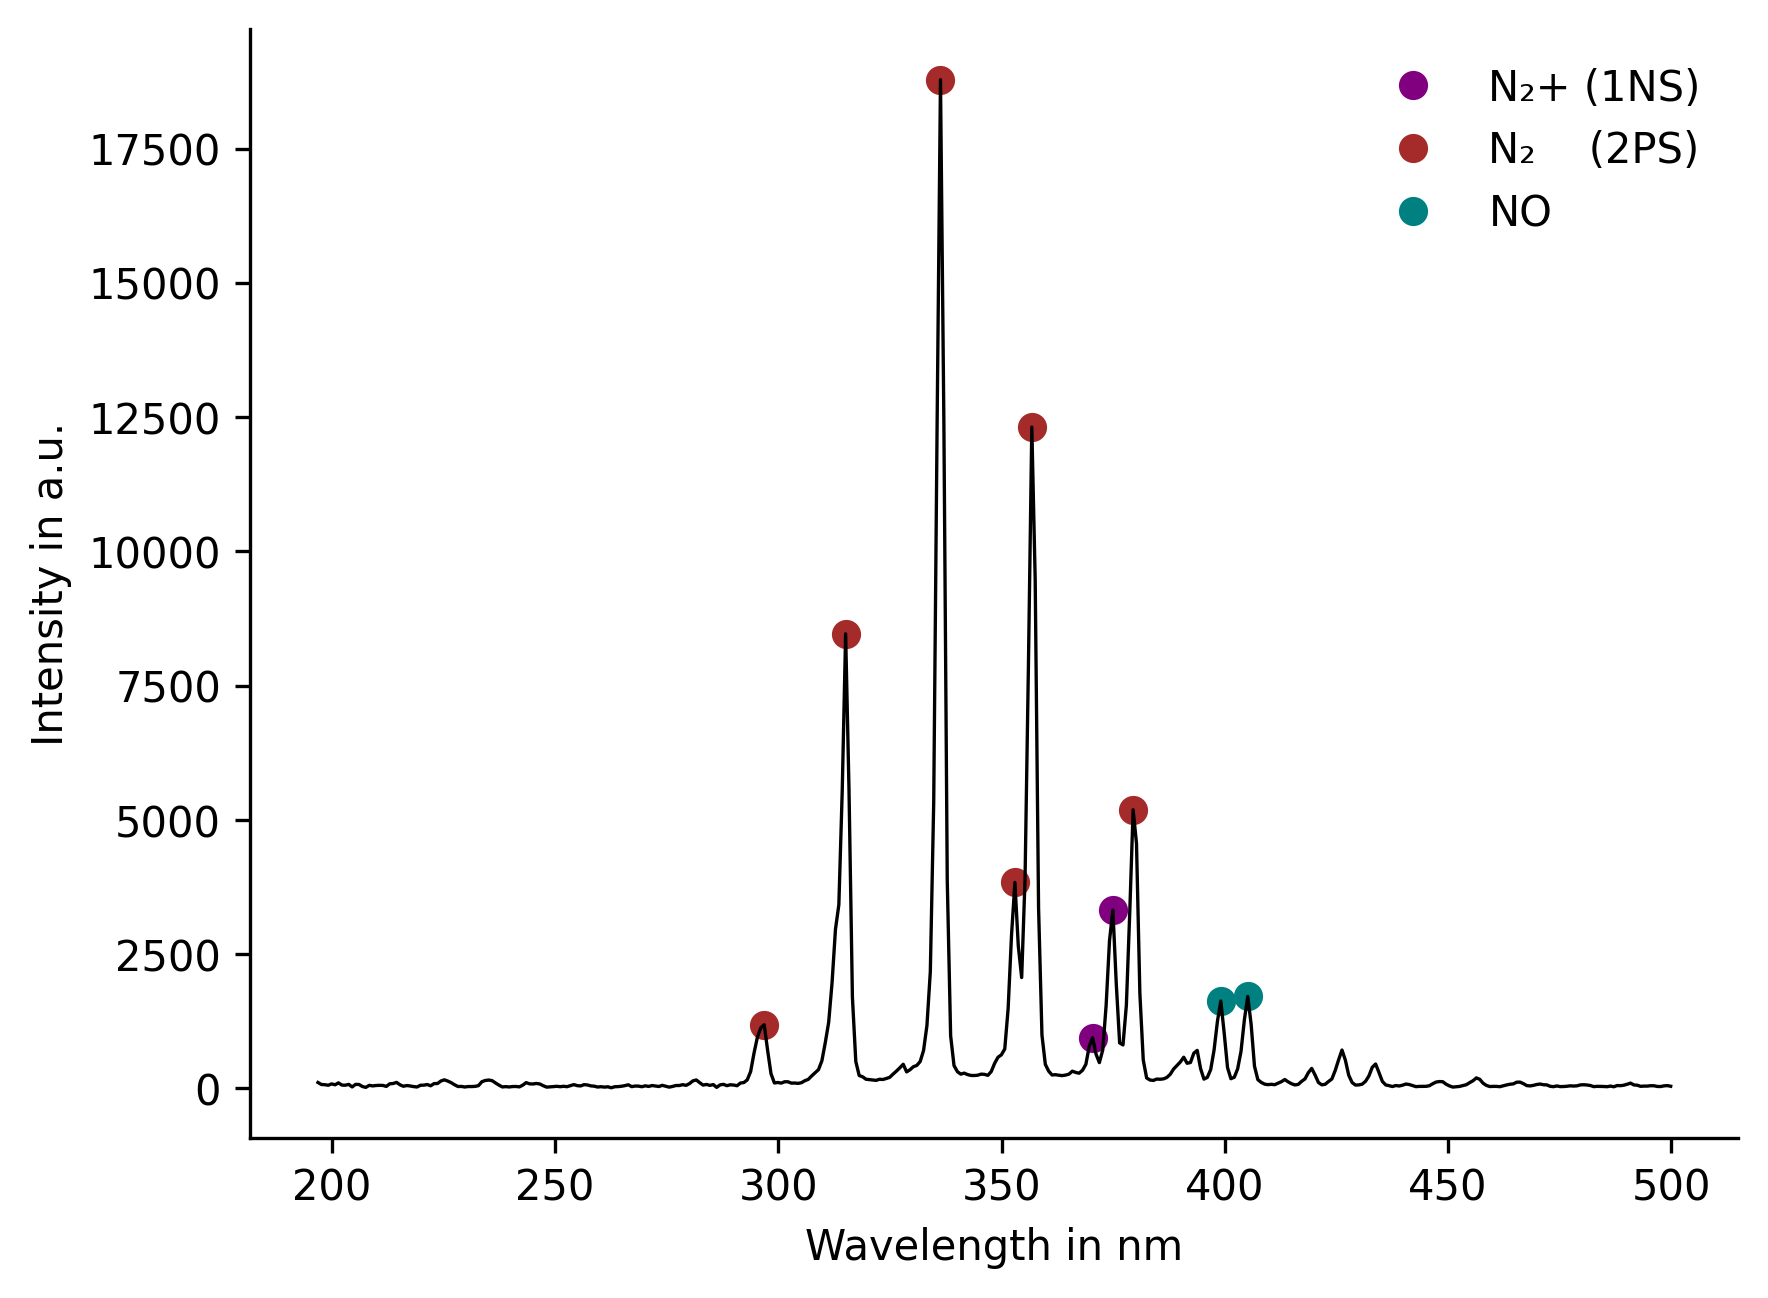
\includegraphics[width=.85\textwidth]{images/OES_analysis.png}
    \caption[OES spectrum with peaks marked]{OES spectrum of the plasma with the peaks marked. The peaks are identified in section \ref{sec:oes_analysis}.}
    \label{fig:oes_analysis}
\end{figure}

\section{Effect of UV Exposure}
To confirm the effect of UV radiation on the spores of C. sphaerospermum, a control experiment is performed. First the spores are exposed to the UV lamp on agar medium for different times. After 15 min of exposure full deactivation was achieved. To control for the effect of the UV light on the agar medium, a second experiment is performed where the agar medium and spores are exposed to the UV light separately. To expose the spores they are instead put into the UV light in water and added to untreated agar media later. In Figure \ref{fig:uv_experiment} the petri dishes after incubation are shown. Table \ref{tab:uv_matrix} shows the number of colonies in a matrix. It becomes clear from this data that the UV light has no significant effect on the agar medium while it has a strong effect on the spores after an exposure time of 15 minutes. Using equation \ref{eq:uv_dose} the dose of UV radiation can be estimated and equates to 1.03 mJ/cm$^2$.

\begin{figure}
    \centering
    \begin{subfigure}[b]{0.6\textwidth}
        \centering
        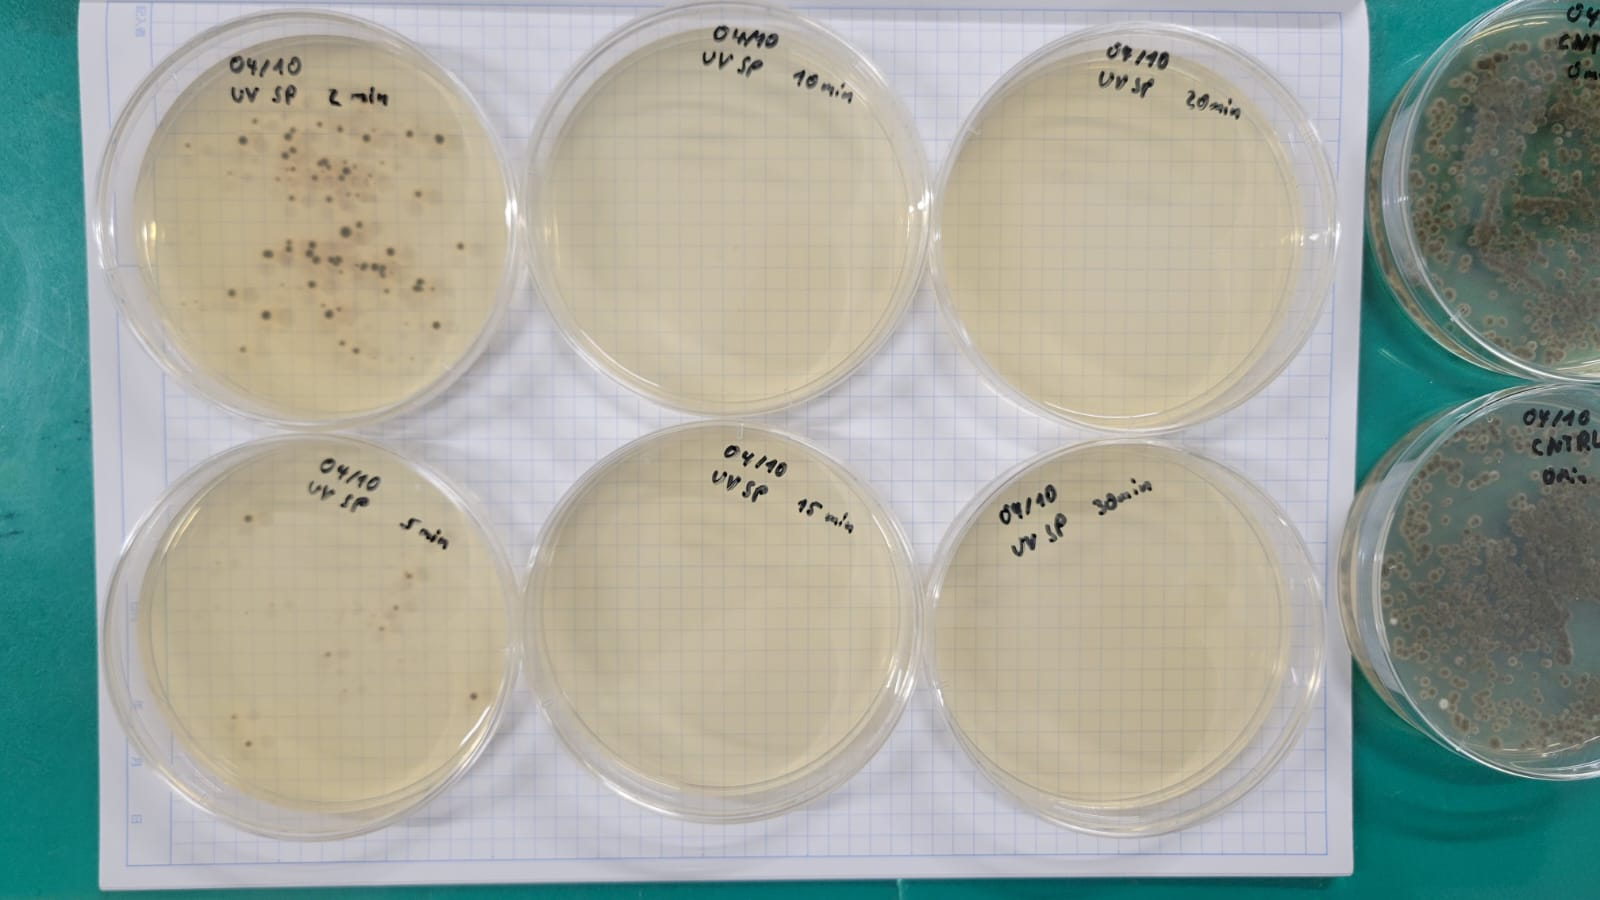
\includegraphics[width=\textwidth]{images/UV_SP.jpeg}
        \caption{Spore UV exposure}
        \label{fig:uv_a}
    \end{subfigure}
    \vfill
    \begin{subfigure}[b]{0.6\textwidth}
        \centering
        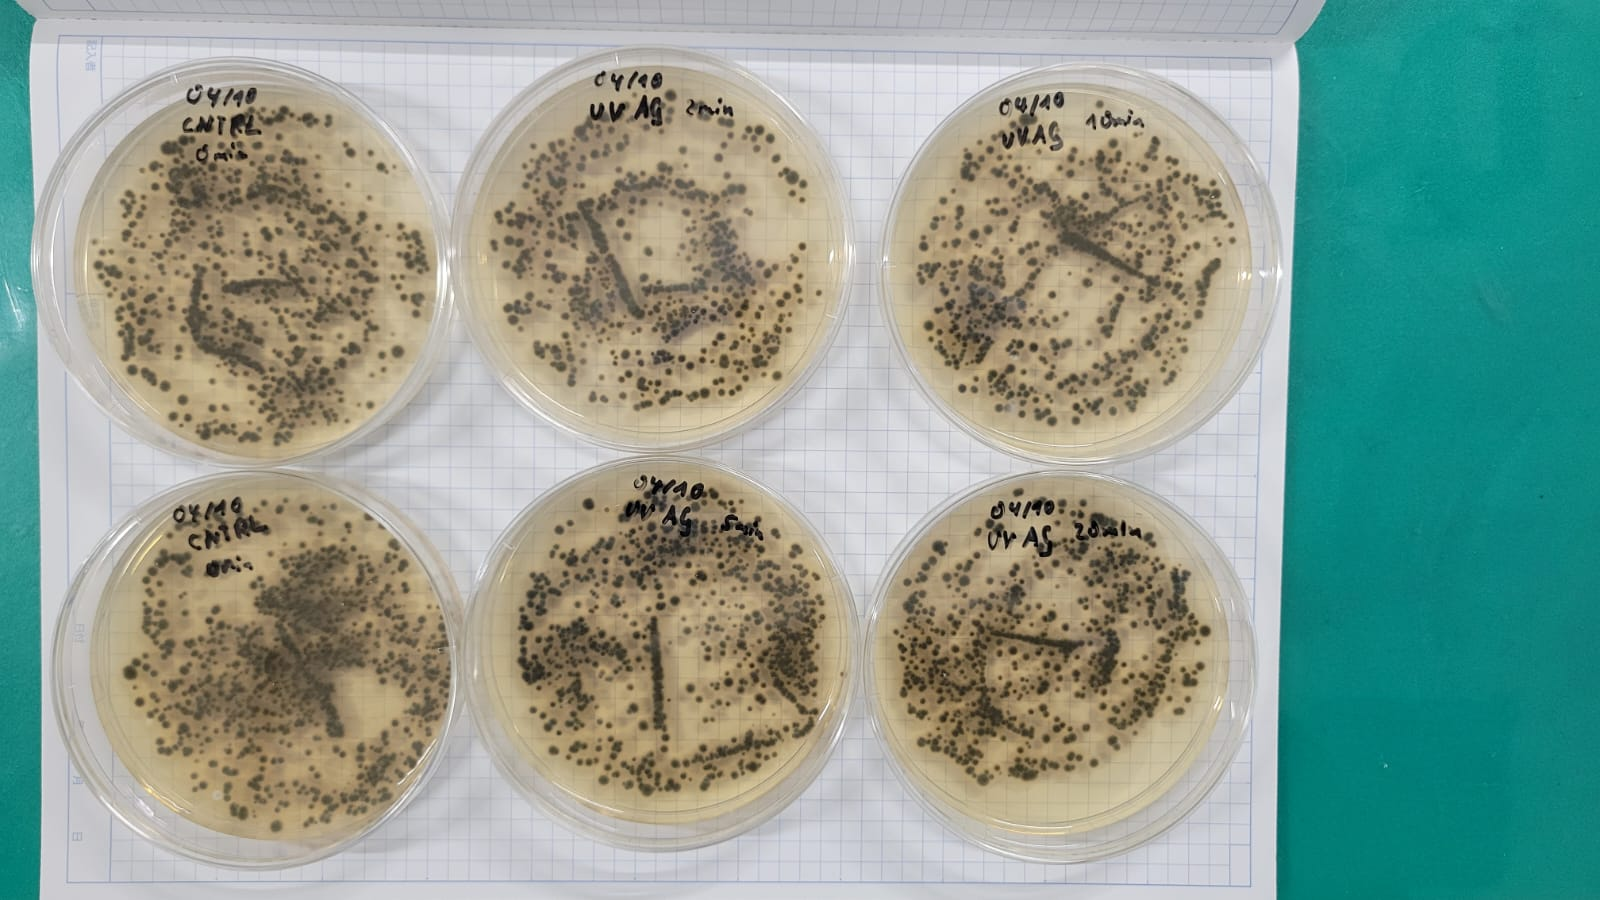
\includegraphics[width=\textwidth]{images/UV_AG.jpeg}
        \caption{Agar UV exposure}
        \label{fig:uv_b}
    \end{subfigure}
    \caption[Photograph of Petri dishes after treatment]{Petri dishes with spores (a) and agar (b) treated with UV light}
    \label{fig:uv_experiment}
\end{figure}

\begin{table}
    \centering
    \caption[Number of colonies after UV exposure as a matrix]{Number of colonies after UV exposure as a matrix. The results after 15 minutes are shown with an estimated dose of ca. 1.03 mJ/cm$^2$.}
    \vspace*{1em}
    \renewcommand{\arraystretch}{1.4}
    \setlength{\tabcolsep}{12pt}
    \begin{tabular}{c|cc}
        {\# of colonies} & {Spores no UV} & {Spores UV} \\
        \hline
        Agar no UV & >100 (cntrl) & 0 \\
        Agar UV    & >100 & 0 \\
    \end{tabular}
    \label{tab:uv_matrix}
\end{table}


\section{Effect of Plasma Treatment}